% meta.concepts: math, 3D vector
% meta.tags: realistic
% inspiration: How to Ace Statics with Jeff Hanson (Test Yourself 1.1, 2023 Edition)i

The City of Rochester installs a sensor atop a lamppost to monitor walking, biking, and car traffic patterns.  To validate the installation, you want to compare the sensor output with measurements made using an alternate reference sensor, as shown in the image.  Write out the position vector from the sensor origin to the:
\begin{itemize}
  \item Fire Hydrant (${\bf r}_{OF}$)
  \item Car Emblem (${\bf r}_{OC}$)
\end{itemize}

\begin{figure}[ht!]
  \centering
  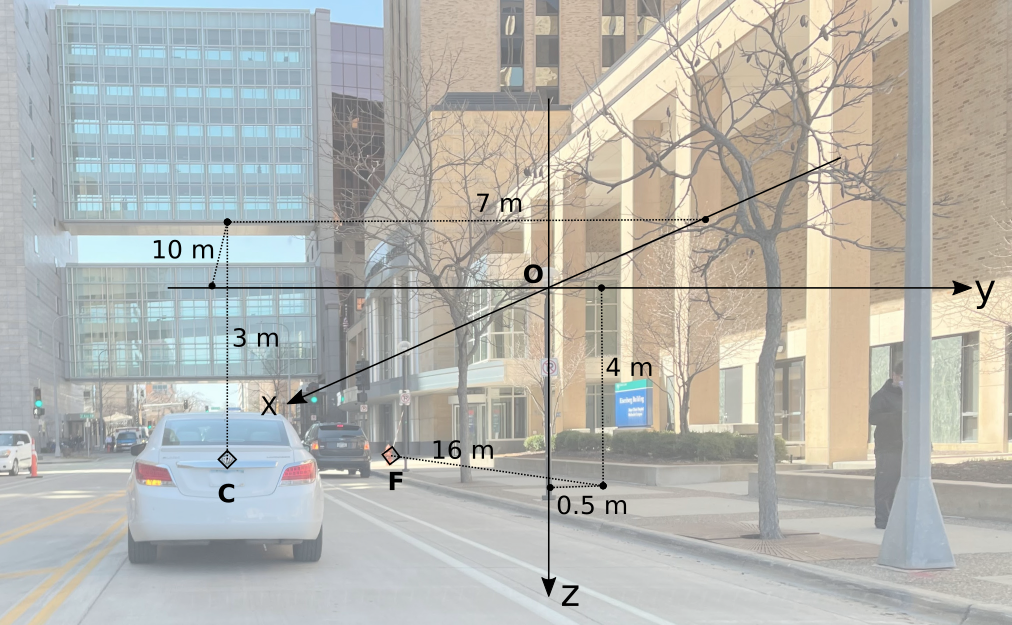
\includegraphics[height=1.8in]{3d-street-buildings.png}
\end{figure}


\vspace{.5cm}
\rule{\textwidth}{.4pt}
\vspace{.5cm}
\textbf{Solution:}
\begin{figure}[ht!]
  \centering
  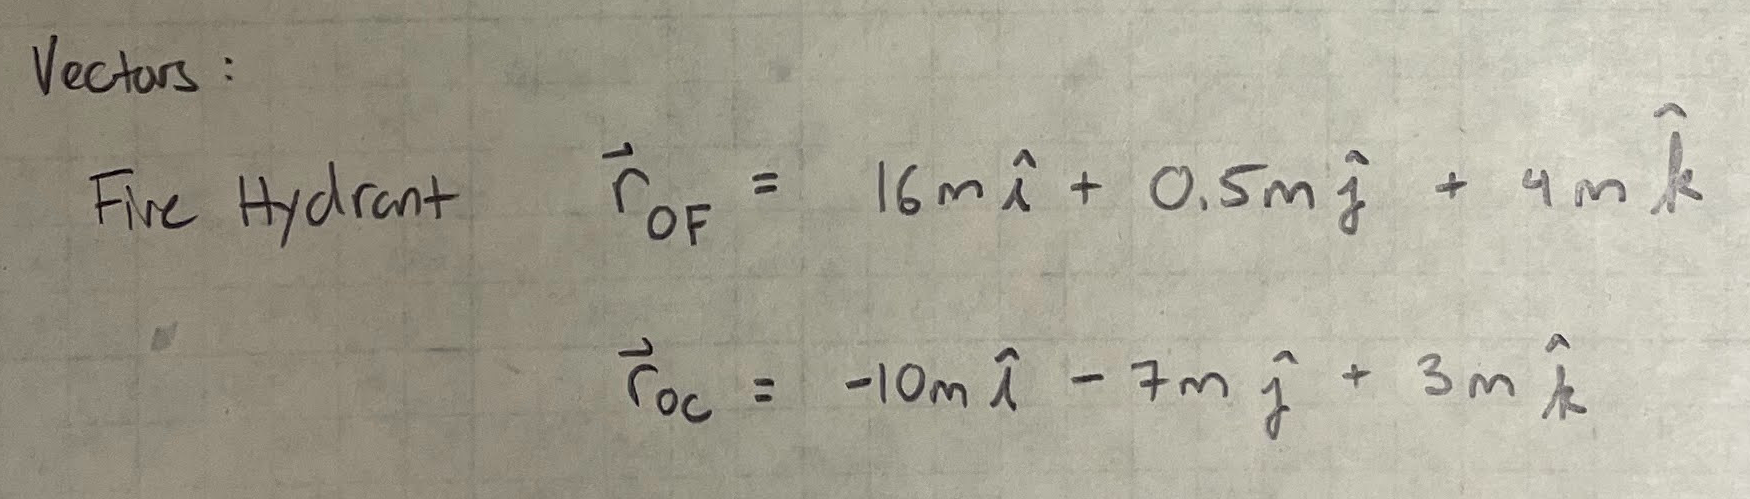
\includegraphics[width=0.9\textwidth]{soln.png}
\end{figure}

